\documentclass[12pt,a4paper]{article}
\usepackage[utf8]{vietnam}
\usepackage{amsmath,amssymb}
\usepackage{geometry}
\geometry{top=1.5cm,bottom=1.2cm,left=1.4cm,right=1.4cm,headheight=28pt,headsep=12pt,footskip=18pt}
\usepackage{tikz}
\usepackage{xcolor}
\usepackage{enumerate}
\usepackage{graphicx}
\usepackage[version=4]{mhchem}
\usepackage{fancyhdr}
\usepackage{ex_test}

\renewcommand{\baselinestretch}{0.96}
\setlength{\parskip}{0pt}

\definecolor{hfRed}{RGB}{211,47,47}
\definecolor{hfGreen}{RGB}{139,195,144}

\pagestyle{fancy}
\fancyhf{}
\fancyhead[L]{\small\itshape\color{hfRed} Tài liệu lưu hành nội bộ}
\fancyhead[R]{\small\itshape\color{hfRed} Thầy \textbf{TRẦN VĂN THẠNH} - 0777.470.803}
\renewcommand{\headrulewidth}{0.8pt}
\renewcommand{\headrule}{\hbox to\headwidth{\color{hfGreen}\leaders\hrule height \headrulewidth\hfill}}

\fancyfoot[L]{\small\itshape\color{hfRed} CS1: 6/15 Nguyễn Hoàng, P. Kim Long, TP Huế \quad|\quad CS2: 24 Đặng Thái Thân, TP Huế}
\fancyfoot[R]{\small\bfseries\color{hfRed} Trang \thepage}
\renewcommand{\footrulewidth}{0.8pt}
\renewcommand{\footrule}{\hbox to\headwidth{\color{hfGreen}\leaders\hrule height \footrulewidth\hfill}}

\fancypagestyle{firstpage}{
  \fancyhf{}
  \renewcommand{\headrulewidth}{0pt}
  \fancyfoot[L]{\small\itshape\color{hfRed} CS1: 6/15 Nguyễn Hoàng, P. Kim Long, TP Huế \quad|\quad CS2: 24 Đặng Thái Thân, TP Huế}
  \fancyfoot[R]{\small\bfseries\color{hfRed} Trang \thepage}
  \renewcommand{\footrulewidth}{0.8pt}
  \renewcommand{\footrule}{\hbox to\headwidth{\color{hfGreen}\leaders\hrule height \footrulewidth\hfill}}
}

\begin{document}
\thispagestyle{firstpage}

\noindent
\begin{minipage}[t]{0.44\textwidth}
	\centering\fontsize{10pt}{12pt}\selectfont
	\textbf{SỞ GIÁO DỤC VÀ ĐÀO TẠO THỪA THIÊN HUẾ}\\
	\textbf{ĐỀ CHÍNH THỨC}\\
	\textit{(Đề thi có 05 trang)}
\end{minipage}\hfill
\begin{minipage}[t]{0.54\textwidth}
	\centering\fontsize{10.5pt}{13pt}\selectfont
	\textbf{ĐỀ KIỂM TRA ĐỊNH KỲ CHƯƠNG 6}\\
	\textbf{(HỢP CHẤT CARBONYL - CARBOXYLIC ACID)}\\
	\textbf{MÔN: HOÁ HỌC - LỚP 11}\\
	\textit{Thời gian làm bài: 50 phút, không kể thời gian phát đề}
	
	\smallskip
	\fbox{\textbf{MÃ ĐỀ: 118}}
\end{minipage}

\smallskip
\noindent\hrulefill
\smallskip

\noindent\textbf{Họ, tên thí sinh:} \dotfill\ \textbf{Lớp:} \dotfill\ \textbf{Số báo danh:} \dotfill

\smallskip
\noindent\textit{(Cho biết nguyên tử khối: H = 1; C = 12; N = 14; O = 16; Na = 23; Mg = 24; Al = 27; P = 31; S = 32; Cl = 35,5; K = 39; Ca = 40; Cr = 52; Mn = 55; Fe = 56; Cu = 64; Zn = 65; Br = 80; Ag = 108; Ba = 137.)}

\smallskip
\noindent\textbf{\large PHẦN I. Câu trắc nghiệm nhiều phương án lựa chọn.}
\textit{Thí sinh trả lời từ câu 1 đến câu 18. Mỗi câu hỏi thí sinh chỉ chọn một phương án.}
\vspace{0.2cm}

\begin{ex}
Gọi tên một hợp chất có công thức cấu tạo như sau: \ce{(CH3)3C-CHO}
\choice
{2-ethyl-2-methylethanal}
{2,2-dimethylpentanal}
{Tert-butyletanal}
{2,2-dimethylpropanal}
\end{ex}

\begin{ex}
Công thức cấu tạo thu gọn của acetone là
\choice
{\ce{OHC-CHO}}
{\ce{CH3COCH3}}
{\ce{CH3CHO}}
{\ce{CH2=CHCHO}}
\end{ex}

\begin{ex}
Tên gọi của aldehyde có khối lượng phân tử nhỏ nhất là
\choice
{aldehyde acetic}
{methanal}
{acetone}
{methanol}
\end{ex}

\begin{ex}
Phản ứng giữa \ce{CH3COCH3} với \ce{HCN} thuộc loại phản ứng
\choice
{phản ứng thuận nghịch}
{phản ứng cộng}
{phản ứng thế}
{phản ứng phân hủy}
\end{ex}

\begin{ex}
Điều kiện của phản ứng giữa aldehyde hoặc ketone với iodine trong dung dịch \ce{NaOH} tạo iodoform là
\choice
{aldehyde hoặc ketone có nhóm methyl cạnh nhóm carbonyl (\ce{CH3CO-})}
{aldehyde hoặc ketone có nhóm methyl cạnh nhóm carbonyl (\ce{C2H3CO-})}
{aldehyde hoặc ketone có nhóm methyl cạnh nhóm carbonyl (\ce{C2H5CO-})}
{aldehyde hoặc ketone có nhóm methyl cạnh nhóm carbonyl (\ce{C3H7CO-})}
\end{ex}

\begin{ex}
\textit{(SBT - CTST)} Cho dãy các chất sau: \ce{HCHO}, \ce{CH3COOH}, \ce{CH3CHO}, \ce{HCOOH}, \ce{C2H5OH}. Số chất trong dãy có thể tham gia phản ứng tráng bạc là
\choice
{3}
{6}
{4}
{5}
\end{ex}

\begin{ex}
\textit{(SBT - CTST)} Có 3 dung dịch: \ce{CH3CHO}, \ce{CH3COOH}, \ce{HCOOH} đựng trong 3 lọ mất nhãn. Hóa chất có thể dùng để phân biệt ba dung dịch trên là
\choice
{quỳ tím, \ce{CuO}}
{quỳ tím, \ce{Na}}
{quỳ tím, dung dịch \ce{AgNO3} trong \ce{NH3} dư}
{dung dịch \ce{AgNO3} trong \ce{NH3} dư, \ce{CuO}}
\end{ex}

\begin{ex}
\textit{(SBT - CD)} Phản ứng nào sau đây thể hiện tính oxi hóa của propanal?
\choice
{\ce{C2H5CHO + 2[Ag(NH3)2]OH -> C2H5COONH4 + 3NH3 + 2Ag v + H2O}}
{\ce{C2H5CHO + Br2 + H2O -> C2H5COOH + 2HBr}}
{\ce{C2H5CHO + 2Cu(OH)2 + NaOH -> C2H5COONa + Cu2O v + 3H2O}}
{\ce{C2H5CHO + 2[H] ->[{LiAlH$_4$}] CH3CH2CH2OH}}
\end{ex}

\begin{ex}
\textit{(SBT - CD)} Khi cho ethanal phản ứng với \ce{Cu(OH)2} trong môi trường kiềm ở nhiệt độ thích hợp, hiện tượng nào sau đây sẽ xảy ra?
\choice
{\ce{Cu(OH)2} bị tan ra, tạo dung dịch màu xanh}
{Có mùi chua của giấm, do phản ứng sinh ra acetic acid}
{Tạo kết tủa đỏ gạch do phản ứng sinh ra \ce{Cu2O}}
{Sinh ra \ce{CuO} màu đen}
\end{ex}

\begin{ex}
Có thể dùng thuốc thử nào trong các chất dưới đây để nhận biết các chất: ethyl alcohol, glycerol, acetic aldehyde đựng trong ba lọ mất nhãn?
\choice
{\ce{Cu(OH)2} trong môi trường kiềm}
{Quỳ tím}
{Kim loại sodium}
{Dung dịch \ce{AgNO3/NH3}}
\end{ex}

\begin{ex}
Có bao nhiêu aldehyde hai chức có công thức đơn giản nhất là \ce{C2H3O}?
\choice
{2}
{4}
{1}
{3}
\end{ex}

\begin{ex}
Có bao nhiêu phản ứng xảy ra khi cho các chất \ce{C6H5OH}, \ce{NaHCO3}, \ce{NaOH}, \ce{HCl} tác dụng với nhau từng đôi một?
\choice
{3}
{4}
{5}
{6}
\end{ex}

\begin{ex}
Cho các hợp chất có công thức sau: \ce{CH3OH}; \ce{CH3CHO}; \ce{HCOOH}; \ce{C2H5NH2}; \ce{C6H6}; \ce{CH3COCH3}; \ce{C2H6}; \ce{C2H5Cl}. Trong các hợp chất trên, có bao nhiêu chất chứa nhóm carbonyl trong phân tử?
\choice
{3}
{4}
{2}
{5}
\end{ex}

\begin{ex}
Quế có vị cay, mùi thơm nồng, được sử dụng phổ biến làm gia vị, vị thuốc trong Đông y. Hợp chất hữu cơ X tạo mùi đặc trưng của quế, có công thức phân tử là \ce{C9H8O}. Trong phân tử X chứa vòng benzene. X tham gia phản ứng tráng bạc và có đồng phân hình học dạng trans. Xác định công thức cấu tạo của X.
\begin{center}
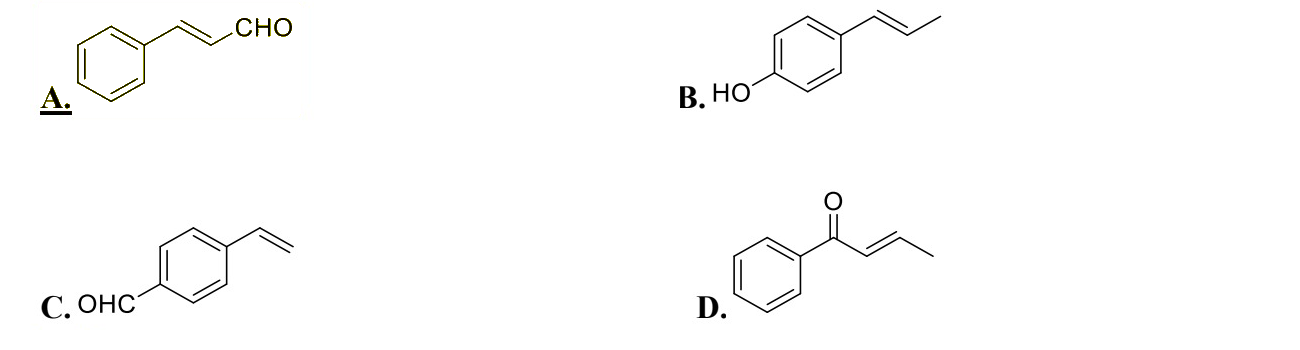
\includegraphics[width=0.88\linewidth]{images_crop_hoa11_de18/c14_grid_student.png}
\end{center}
\choice
{Phương án A}
{Phương án B}
{Phương án C}
{Phương án D}
\end{ex}

\begin{ex}
Một thí nghiệm được mô tả như hình sau đây:
\begin{center}
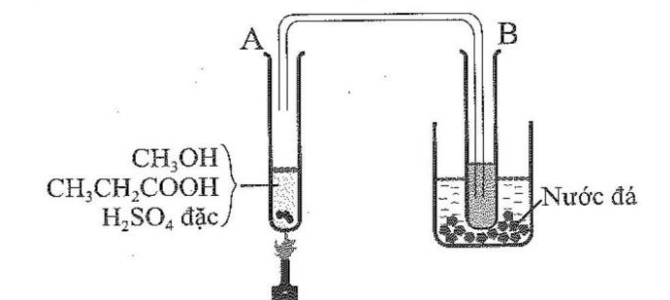
\includegraphics[width=0.48\linewidth]{images_crop_hoa11_de18/c15_experiment.png}
\end{center}
Chất lỏng thu được ở ống nghiệm B có mùi táo, có tên gọi là
\choice
{ethyl formate}
{methyl propionate}
{ethyl propionate}
{propyl formate}
\end{ex}

\begin{ex}
Cho giá trị $K_{\text{a}}$ của một số carboxylic acid ở 25 $^\circ$C dưới đây:
\begin{center}
\begin{tabular}{|l|c|c|c|c|}
\hline
\textbf{Carboxylic acid} & \ce{HCOOH} & \ce{CH3COOH} & \ce{CH3CH2COOH} & \ce{C6H5COOH} \\ \hline
$K_{\text{a}}$ & $17,72 \times 10^{-5}$ & $1,75 \times 10^{-5}$ & $1,35 \times 10^{-5}$ & $6,25 \times 10^{-5}$ \\ \hline
\end{tabular}
\end{center}
Tính acid của carboxylic acid nào là mạnh nhất?
\choice
{\ce{HCOOH}}
{\ce{CH3COOH}}
{\ce{CH3CH2COOH}}
{\ce{C6H5COOH}}
\end{ex}

\begin{ex}
\textit{(SBT - CD)} Để trung hòa 40 mL giấm ăn cần 25 mL dung dịch \ce{NaOH} 1 M. Biết khối lượng riêng của giấm ăn xấp xỉ là 1 g/mL. Mẫu giấm ăn này có nồng độ phần trăm là
\choice
{3,5\%}
{3,75\%}
{4\%}
{5\%}
\end{ex}

\begin{ex}
Đun 12 gam acetic acid với một lượng dư ethanol (\ce{H2SO4} đặc làm xúc tác). Đến khi dừng thí nghiệm thu được 8,36 gam ester. Hiệu suất của phản ứng ester hóa là
\choice
{65,15\%}
{54,54\%}
{34,84\%}
{47,50\%}
\end{ex}

\vspace{0.3cm}
\noindent\textbf{\large PHẦN II. Câu trắc nghiệm đúng sai.}
\textit{Thí sinh trả lời từ câu 1 đến câu 4. Trong mỗi ý a), b), c), d) ở mỗi câu, thí sinh chọn đúng hoặc sai.}
\vspace{0.2cm}

\begin{ex}
Muscone là hợp chất tạo nên mùi thơm đặc trưng của xạ hương, có công thức cấu tạo như sau:
\begin{center}
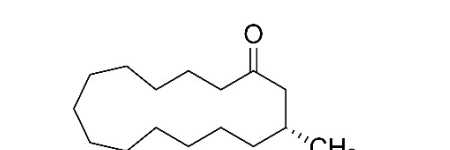
\includegraphics[width=0.35\linewidth]{images_crop_hoa11_de18/muscone.png}
\end{center}
\choiceTF
{Muscone thuộc hợp chất ketone}
{Muscone có công thức phân tử là \ce{C16H30O}}
{Muscone có thể tham gia phản ứng tráng bạc với thuốc thử Tollens}
{Muscone có nhiệt độ sôi cao hơn so với ethanal}
\end{ex}

\begin{ex}
Trong nọc độc của một số côn trùng như kiến, ong, muỗi... có chứa hợp chất acid X gây bỏng rát và ngứa.
\choiceTF
{X là acetic acid, có công thức cấu tạo là \ce{CH3COOH}}
{X là formic acid, có công thức phân tử là \ce{HCOOH}}
{Khi bị côn trùng đốt thì nên bôi vôi vào vết côn trùng đốt nó sẽ trung hòa lượng acid X làm cho vết đốt đỡ ngứa rát: \ce{2HCOOH + Ca(OH)2 -> (HCOO)2Ca + 2H2O}}
{Cho dung dịch acid X vào ống nghiệm chứa dung dịch \ce{AgNO3/NH3}, sau đó đun nóng nhẹ thì thấy thành ống nghiệm sáng bóng như gương}
\end{ex}

\begin{ex}
Tiến hành phản ứng tráng bạc aldehyde acetic với thuốc thử Tollens theo các bước sau đây:\\
\textit{Bước 1:} Rửa sạch ống nghiệm bằng cách nhỏ vài giọt dung dịch kiềm \ce{NaOH}, đun nóng nhẹ, tráng đều, sau đó đổ đi và tráng lại bằng nước cất.\\
\textit{Bước 2:} Nhỏ vào ống nghiệm 2 giọt dung dịch \ce{AgNO3} và 1 giọt dung dịch \ce{NH3}, xuất hiện kết tủa nâu xám, nhỏ tiếp dung dịch \ce{NH3} đến khi kết tủa tan hết.\\
\textit{Bước 3:} Nhỏ tiếp vào ống nghiệm 2 giọt dung dịch \ce{CH3CHO}.\\
\textit{Bước 4:} Lắc đều ống nghiệm, đun cách thủy (trong cốc nước nóng) vài phút ở 60 -- 70 $^\circ$C.
\choiceTF
{Sau bước 4 quan sát thấy thành ống nghiệm sáng bóng như gương}
{Ở bước 3 nếu thay aldehyde acetic bằng acetone thì thu được hiện tượng tương tự}
{Ở bước 4 xảy ra phản ứng oxi hóa -- khử trong đó aldehyde acetic là chất bị khử}
{Sản phẩm hữu cơ thu được trong dung dịch sau bước 4 có công thức phân tử là \ce{C2H7NO2}}
\end{ex}

\begin{ex}
Hãy chọn các nhận định về hiện tượng và phương trình hóa học xảy ra đúng trong các trường hợp sau:
\choiceTF
{Cho acetic aldehyde tác dụng với nước bromine thấy nước bromine bị mất màu do xảy ra phản ứng: \ce{CH3CHO + Br2 + H2O -> CH3COOH + 2HBr}}
{Cho formic aldehyde tác dụng với dung dịch \ce{AgNO3} trong \ce{NH3} dư thấy xuất hiện kết tủa trắng sáng do xảy ra phản ứng: \ce{HCHO + 4[Ag(NH3)2]OH ->[{t$^\circ$}] (NH4)2CO3 + 4Ag v + 6NH3 + 2H2O}}
{Cho acetone tác dụng với \ce{I2} trong dung dịch \ce{NaOH} dư không có hiện tượng gì xảy ra}
{Cho acetic aldehyde tác dụng với \ce{Cu(OH)2} trong \ce{NaOH} dư thấy xuất hiện kết tủa đỏ gạch do xảy ra phản ứng: \ce{C2H5CHO + 2Cu(OH)2 + NaOH ->[{t$^\circ$}] C2H5COONa + Cu2O v + 3H2O}}
\end{ex}

\vspace{0.3cm}
\noindent\textbf{\large PHẦN III. Câu trắc nghiệm yêu cầu trả lời ngắn.}
\textit{Thí sinh trả lời từ câu 1 đến câu 6.}
\vspace{0.2cm}

\begin{ex}
Cho các hóa chất sau: dung dịch \ce{HCN}, dung dịch \ce{Br2}, dung dịch \ce{NaOH}, dung dịch \ce{[Ag(NH3)2]OH}, \ce{LiAlH4}, \ce{Cu(OH)2/NaOH}, \ce{I2/NaOH}. Có bao nhiêu chất phản ứng được với acetone ở điều kiện nhiệt độ thích hợp?

\vspace{0.2cm}
\noindent\textbf{Đáp số:} \dotfill
\end{ex}

\begin{ex}
Aldehyde (X) no, đơn chức, mạch hở không nhánh. Phân tử khối của (X) được xác định thông qua kết quả phổ khối lượng với peak ion phân tử có giá trị $m/z$ lớn nhất trong hình dưới đây. Khối lượng mol của X là bao nhiêu g/mol?
\begin{center}
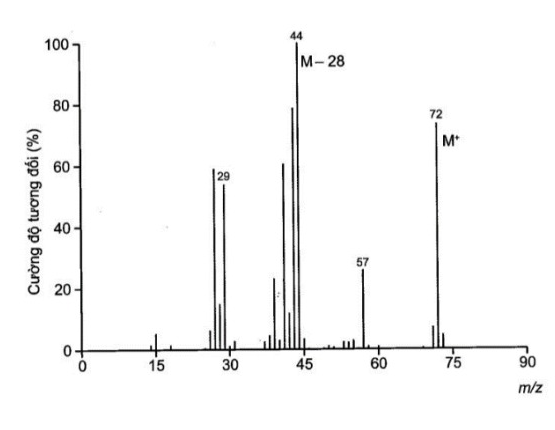
\includegraphics[width=0.45\linewidth]{images_crop_hoa11_de18/ms_spectrum.png}
\end{center}

\vspace{0.2cm}
\noindent\textbf{Đáp số:} \dotfill
\end{ex}

\begin{ex}
Cho các chất sau: \ce{Cu}, \ce{Na}, \ce{Mg}, \ce{KOH}, \ce{Na2CO3}, \ce{NaCl}, \ce{HCOOH}, \ce{C2H5OH}. Có bao nhiêu chất phản ứng được với \ce{CH3COOH}?

\vspace{0.2cm}
\noindent\textbf{Đáp số:} \dotfill
\end{ex}

\begin{ex}
Hợp chất carboxylic acid X có công thức đơn giản nhất là \ce{CH2O}. Phổ MS cho thấy X có các tín hiệu sau:
\begin{center}
\begin{tabular}{|c|c|}
\hline
\textbf{$m/z$} & \textbf{Cường độ tương đối (\%)} \\ \hline
29 & 19 \\ \hline
31 & 100 \\ \hline
60 & 39 \\ \hline
\end{tabular}
\end{center}
Biết mảnh $[\text{M}^+]$ có giá trị $m/z$ lớn nhất. Tổng số nguyên tử trong một phân tử của X là bao nhiêu?

\vspace{0.2cm}
\noindent\textbf{Đáp số:} \dotfill
\end{ex}

\begin{ex}
Nước ép chanh chứa khoảng 5\% (khoảng 0,3 mol/lít) citric acid, điều này giúp chanh có vị chua và độ pH từ 2 -- 3. Citric acid có công thức cấu tạo là:
\begin{center}
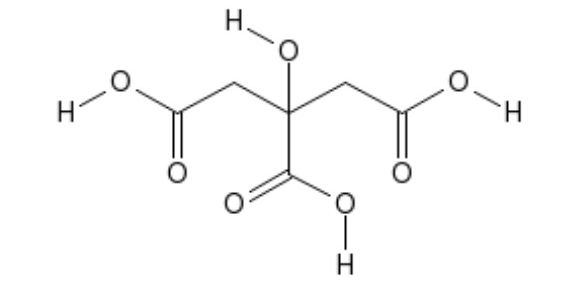
\includegraphics[width=0.35\linewidth]{images_crop_hoa11_de18/citric_acid.png}
\end{center}
Phân tử khối của citric acid là bao nhiêu amu?

\vspace{0.2cm}
\noindent\textbf{Đáp số:} \dotfill
\end{ex}

\begin{ex}
Thực hiện phản ứng oxi hóa 4,958 L \ce{C2H4} (đkc) bằng \ce{O2} (xúc tác \ce{PdCl2}, \ce{CuCl2}) thu được chất X đơn chức. Cho toàn bộ lượng chất X tác dụng với hydrogen cyanide (\ce{HCN}) dư, thu được 7,1 gam \ce{CH3CH(CN)OH} (cyanohydrin). Hiệu suất của quá trình tạo \ce{CH3CH(CN)OH} từ \ce{C2H4} là $x$\%. Giá trị của $x$ là bao nhiêu?

\vspace{0.2cm}
\noindent\textbf{Đáp số:} \dotfill
\end{ex}

\vspace{0.3cm}
\noindent\textbf{\large PHẦN IV. Tự luận.}
\textit{Thí sinh trình bày bài giải chi tiết vào giấy làm bài.}
\vspace{0.2cm}

\begin{ex}
\textit{(1,0 điểm)} Hoàn thành dãy chuyển hóa sau bằng các phương trình hóa học:
$$\ce{Ethane ->[(1)] Ethyl chloride ->[(2)] Ethanol ->[(3)] Ethanal ->[(4)] Acetic acid}$$

\vspace{0.2cm}
\noindent\dotfill\\[4pt]
\noindent\dotfill\\[4pt]
\noindent\dotfill\\[4pt]
\noindent\dotfill\\[4pt]
\noindent\dotfill
\end{ex}

\begin{ex}
\textit{(1,0 điểm)} Để xác định được hợp chất hữu cơ X, người ta thực hiện các phân tích sau:\\
-- Bằng phương pháp phân tích nguyên tố, xác định được X chứa \%C = 40,0\%; \%H = 6,67\%, còn lại là oxygen.\\
-- Bằng phương pháp đo phổ MS, kết quả cho thấy trên phổ xuất hiện peak ion phân tử $[\text{M}^+]$ có giá trị $m/z$ bằng 60.\\
-- Bằng phương pháp đo phổ IR, kết quả cho thấy trên phổ xuất hiện peak rộng trong vùng từ 2 500 đến 3 200 cm$^{-1}$, và một peak hấp thụ mạnh ở 1 745 cm$^{-1}$.\\
Xác định công thức phân tử và công thức cấu tạo thu gọn của hợp chất X.

\vspace{0.2cm}
\noindent\dotfill\\[4pt]
\noindent\dotfill\\[4pt]
\noindent\dotfill\\[4pt]
\noindent\dotfill\\[4pt]
\noindent\dotfill
\end{ex}

\bigskip
\begin{center}
\textbf{---------- HẾT ----------}
\end{center}
\end{document}
